\documentclass{article}
\usepackage[T1]{fontenc}
\usepackage[utf8]{inputenc}
\usepackage[french]{babel}
\usepackage{listings, xcolor, graphicx}
\usepackage{amsmath}
\usepackage{textgreek}
\usepackage{enumitem}
\usepackage{subcaption}
\graphicspath{ {./} }

\title{Modélisation de la propagation des variants du COVID}
\author{BOUZAKRI Wassim \\COUPET Joss \\MARCHETTI Marie-Eden \\VASSEUR Pierre-Adrien}
\date{Février 2022}

\begin{document}

\maketitle

\section{Résumé}

Dans ce rapport, on a répondu a la problématique suivante :\\
Le comportement de l'épidemie de la COVID-19 est-il influencé par la circulation, la mutation et l'interaction de variants ?
Pour répondre à cette question, on a mis en place un certain nombre d'équation afin de réaliser des simulations. \\Celles-ci nous ont permis d'en conclure que la circulation, la mutation et l'interaction influencent le comportement de l'épidemie.

\section{Introduction}

Dans ce rapport, on va étudier la propagation de la COVID-19 par le biais des variants.
On se demande alors si leur circulation et mutation influencent le comportement de l'épidémie, en plus de considérer leur interaction entre eux.\\

\noindent
Concernant les recherches existantes, on a découvert peu d'articles présentant des simulations de propagation de la Covid-19 par le biais des variants.
Les quelques articles existants se concentraient surtout des propriétés biologiques du virus influencant la simulation de la mutation et la propagation.
Par exemple, la taille du génome du virus parent ou les symptômes. (Marquioni \& de Aguiar, 2021), ce sont des analyses intéressantes mais sans doute trop complexe sans avoir suivi la formation adéquate.\\

\noindent
Une approche différente et plus simple a été choisie afin de permettre la compréhension par un maximum de lecteurs. Elle sere détaillée tout au long de cet article.\\

\noindent
Tout d'abord, on présentera la modélisation de départ de la propagation de la Covid-19 initialisée avec un seul variant. \par
Ensuite, on se penchera sur la modélisation plus complexe initialisée avec deux variants, sur lequel on concentra notre étude.\par
Puis, on réalisera plusieurs simulations différentes dans l'objectif d'interpréter le comportement de ce modèle grâce aux résultats.\par
Enfin, on concluera notre étude.\\

\section{Modélisation de départ}

La modélisation de départ est très basique et représente l'évolution d'un seul variant en prenant en compte sa virulence et sa force de contamination.\\
\noindent
Les variables de base pour seulement 1 virus sont les suivantes :
\begin{align}
    S(t)= \text{\% de personnes saines dans la population au temps t} \\
    I(t)= \text{\% de personnes contaminées dans la population au temps t} \\
    R(t)= \text{\% de personnes en rémission dans la population au temps t} \\
\end{align}
\noindent
\textalpha \space représente la force de contagion du virus. \\
\textbeta \space représente la virulence du virus. \\
\noindent
La simulation discrétisée par le temps est représentée dans le système d'équation suivante :
\begin{align}
    \dot{S}(t)= -\alpha S(t)I(t) \\
    \dot{I}(t)= \alpha S(t)I(t)-\beta I(t) \\
    \dot{R}(t)= \beta I(t) + \beta I(t)
\end{align}
\noindent
Cette mise en équation permet de simuler facilement la propagation de la Covid-19 au sein d'une population saine.\\

\section{Modélisation avancée}

Afin de modéliser un modèle à X variants, un nouveau système d'équation est nécessaire.\\
Pour débuter, on a définit un nouveau modèle avec 2 variants qui pourra être modifié pour permettre de simuler X variants.\\
\noindent
Les variables de notre nouveau modèle sont les mêmes que précédemment, c'est-à-dire :
\begin{align}
    S_1(t)= \text{\% de non infecté par le variant 1.} \\
    S_2(t)= \text{\% de non infecté par le variant 2.} \\
    I_1(t)= \text{\% d'infecté au variant 1.} \\
    I_2(t)= \text{\% d'infecté au variant 2.} \\
    R_1(t)= \text{\% de remis au variant 1.} \\
    R_2(t)= \text{\% de remis au variant 2.} \\
\end{align}
\noindent
On obtient donc 2 systèmes d'équations différents. \\
\noindent
Le premier système d'équation est celui qui permet de simuler l'évolution du premier variant.\\
\begin{align}
    \dot{S_1}(t)= -\alpha_1 S_1(t)I_1(t) \\
    \dot{I_1}(t)= \alpha_1 S_1(t)I_1(t)-\beta_1 I_1(t) \\
    \dot{R_1}(t)= \beta_1 I_1(t)
\end{align}
On obtient le même pour le second variant. \\
Cependant le système est trop simple, il n'y a pas d'interaction entre les virus. \\
On fait donc un nouveau système qui permet une interaction entre les variants et qui sera adaptable à X variants à l'aide de boucle en programmation :
\begin{align}
    \dot{S}(t)= -\alpha_1 S(t)I_1(t) - \alpha_2 S(t)I_2(t) \\
    \dot{I_1}(t)= \alpha_1 S(t)I_1(t)-\beta_1 I_1(t) \\
    \dot{I_2}(t)= \alpha_2 S(t)I_2(t)-\beta_2 I_2(t) \\
    \dot{R}(t)= \beta_1 I_1(t) + \beta_2 I_2(t)
\end{align}
\noindent
Lors de la création de ce modèle, on a définit les règles suivante : \\
\begin{enumerate}
    \item On ne peut être infecté que par un variant à la fois. \\
    \item Après s'être remis, on ne peut plus être infecté par un variant. \\
\end{enumerate}

\noindent
On veut maintenant modéliser les mutations.\\
Le \% de chance de mutation du variant 1 sur l'intervalle de temps T est défini par :
\begin{align}
    mut = I_1(t)*(1-e^{\gamma T})\text{ avec }\gamma > \text{0}
\end{align}
\noindent
Si une mutation doit être réalisé alors \\
\noindent
T est un nombre aléatoire tel que 0 < T < 100 \\
t est la probabilité que les propriétés d'un variant soient fortement différentes des propriétés du parent.\\
Si T > t \\
Alors F(T) =
\begin{align}
    new_\alpha = x, \alpha_{variant} \times 1.2 < x < \alpha_{variant} \times 1.4 \\
    new_\beta = x, \beta_{variant} \times 0.9 < x < \beta_{variant} \times 1.1
\end{align}
\noindent
Sinon F(T) = \\
\begin{align}
    new_\alpha= x, \alpha_{variant} \times 0.1 < x < \alpha_{variant} \times 1.9 \\
    new_\beta= x, \beta_{variant} \times 0.1 < x < \beta_{variant} \times 1.9
\end{align}


\section{Simulations numériques}

Dans cette partie, on va réaliser plusieurs simulations avec différents paramètres. Ces simulations sont produites avec un outil que l'on a développé et déployé en ligne, disponible à l'adresse suivante : https://modelisation.vercel.app/ \\
Les paramètres initiaux sont les suivants : \\
\begin{enumerate}
    \item Taux de personnes saines = 0,97
    \item Taux de personnes en rémission = 0
    \item Mutabilité du virus = 0,01
    \item Probabilité de créer un nouveau variant avec des paramètres très éloignées de son parent = 1
    \item Durée de la simulation en jours = 2000\\
\end{enumerate}
Pour le variant 1 :
\begin{enumerate}
    \item Taux de personnes infecté = 0,01
    \item Force de contagion du variant = 0,01
    \item Virulence du variant = 0,001\\
\end{enumerate}
Pour le variant 2 :
\begin{enumerate}
    \item Taux de personnes infecté = 0,02
    \item Force de contagion du variant = 0,01
    \item Virulence du variant = 0,005\\
\end{enumerate}

Dans la majorité des simulations, on fera varier un seul de ses paramètres afin d'identifier la cause réel du changement. \\
Si on se permet de modifier plusieurs paramètres en même temps, on ne peut plus être sûr de ce qui cause un possible changement observé. \\

\subsection{Simulation de référence}

\begin{figure}[h]
    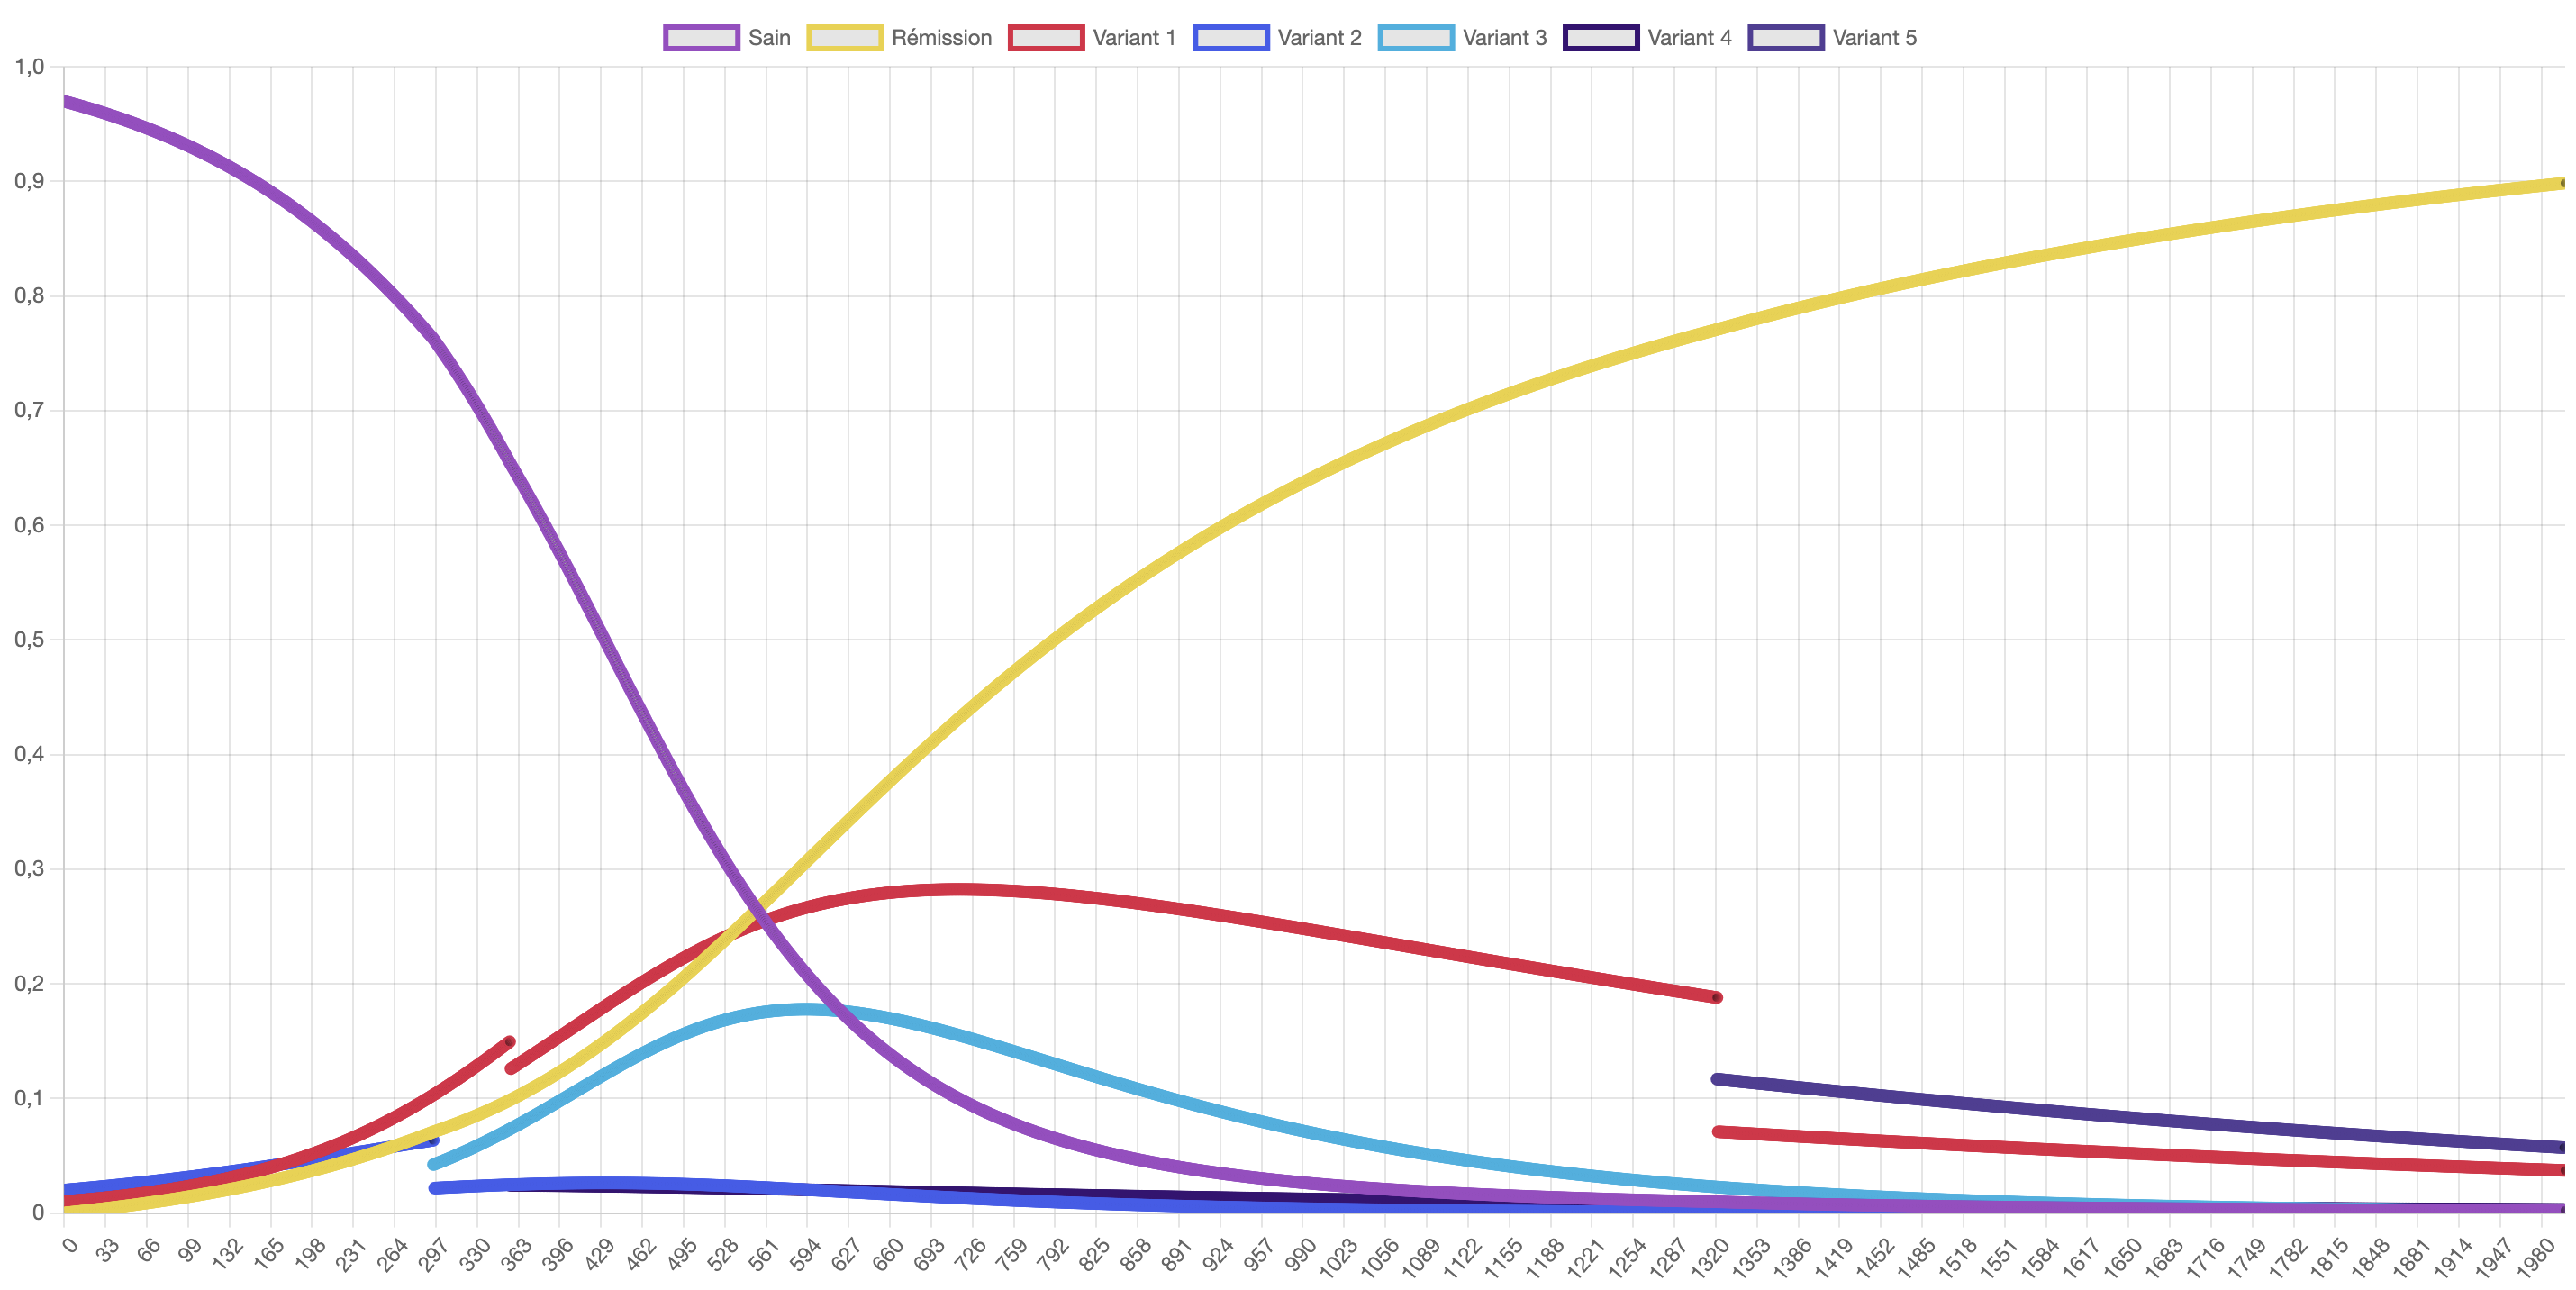
\includegraphics[width=\linewidth]{images/Simulation1.png}
    \caption{Simulation de référence}
    \label{fig:simulation1}
\end{figure}

\noindent
La simulation de référence utilise les paramètres de base énoncé un peu plus haut. \\
On remarque la création de 6 nouveaux variants : \\
\begin{enumerate}
    \item Variant 3 : Apparition au jour 231. Il est issu du variant 2. Il ne survit pas.
    \item Variant 4 : Apparition au jour 561. Il est issu du variant 1.
    \item Variant 5 : Apparition au jour 627. Il est issu du variant 4. Il survit avec un faible taux d'infection.
    \item Variant 6 : Apparition au jour 660. Il est issu du variant 2. Il ne survit pas.
    \item Variant 7 : Apparition au jour 1419. Il est issu du variant 4. Il ne survit pas.
    \item Variant 8 : Apparition dans les derniers jours de la modélisation.
\end{enumerate}

On remarque que quasiment tout les variants sont dérivés du variant 3 ou d'un de ses enfants. Explication ? Naissance avec des caractéristiques très dfférentes de son parent. \\

\subsection{Influence de la mutabilité du virus}

\begin{figure}[h]
  \begin{subfigure}{.5\textwidth}
  \centering
  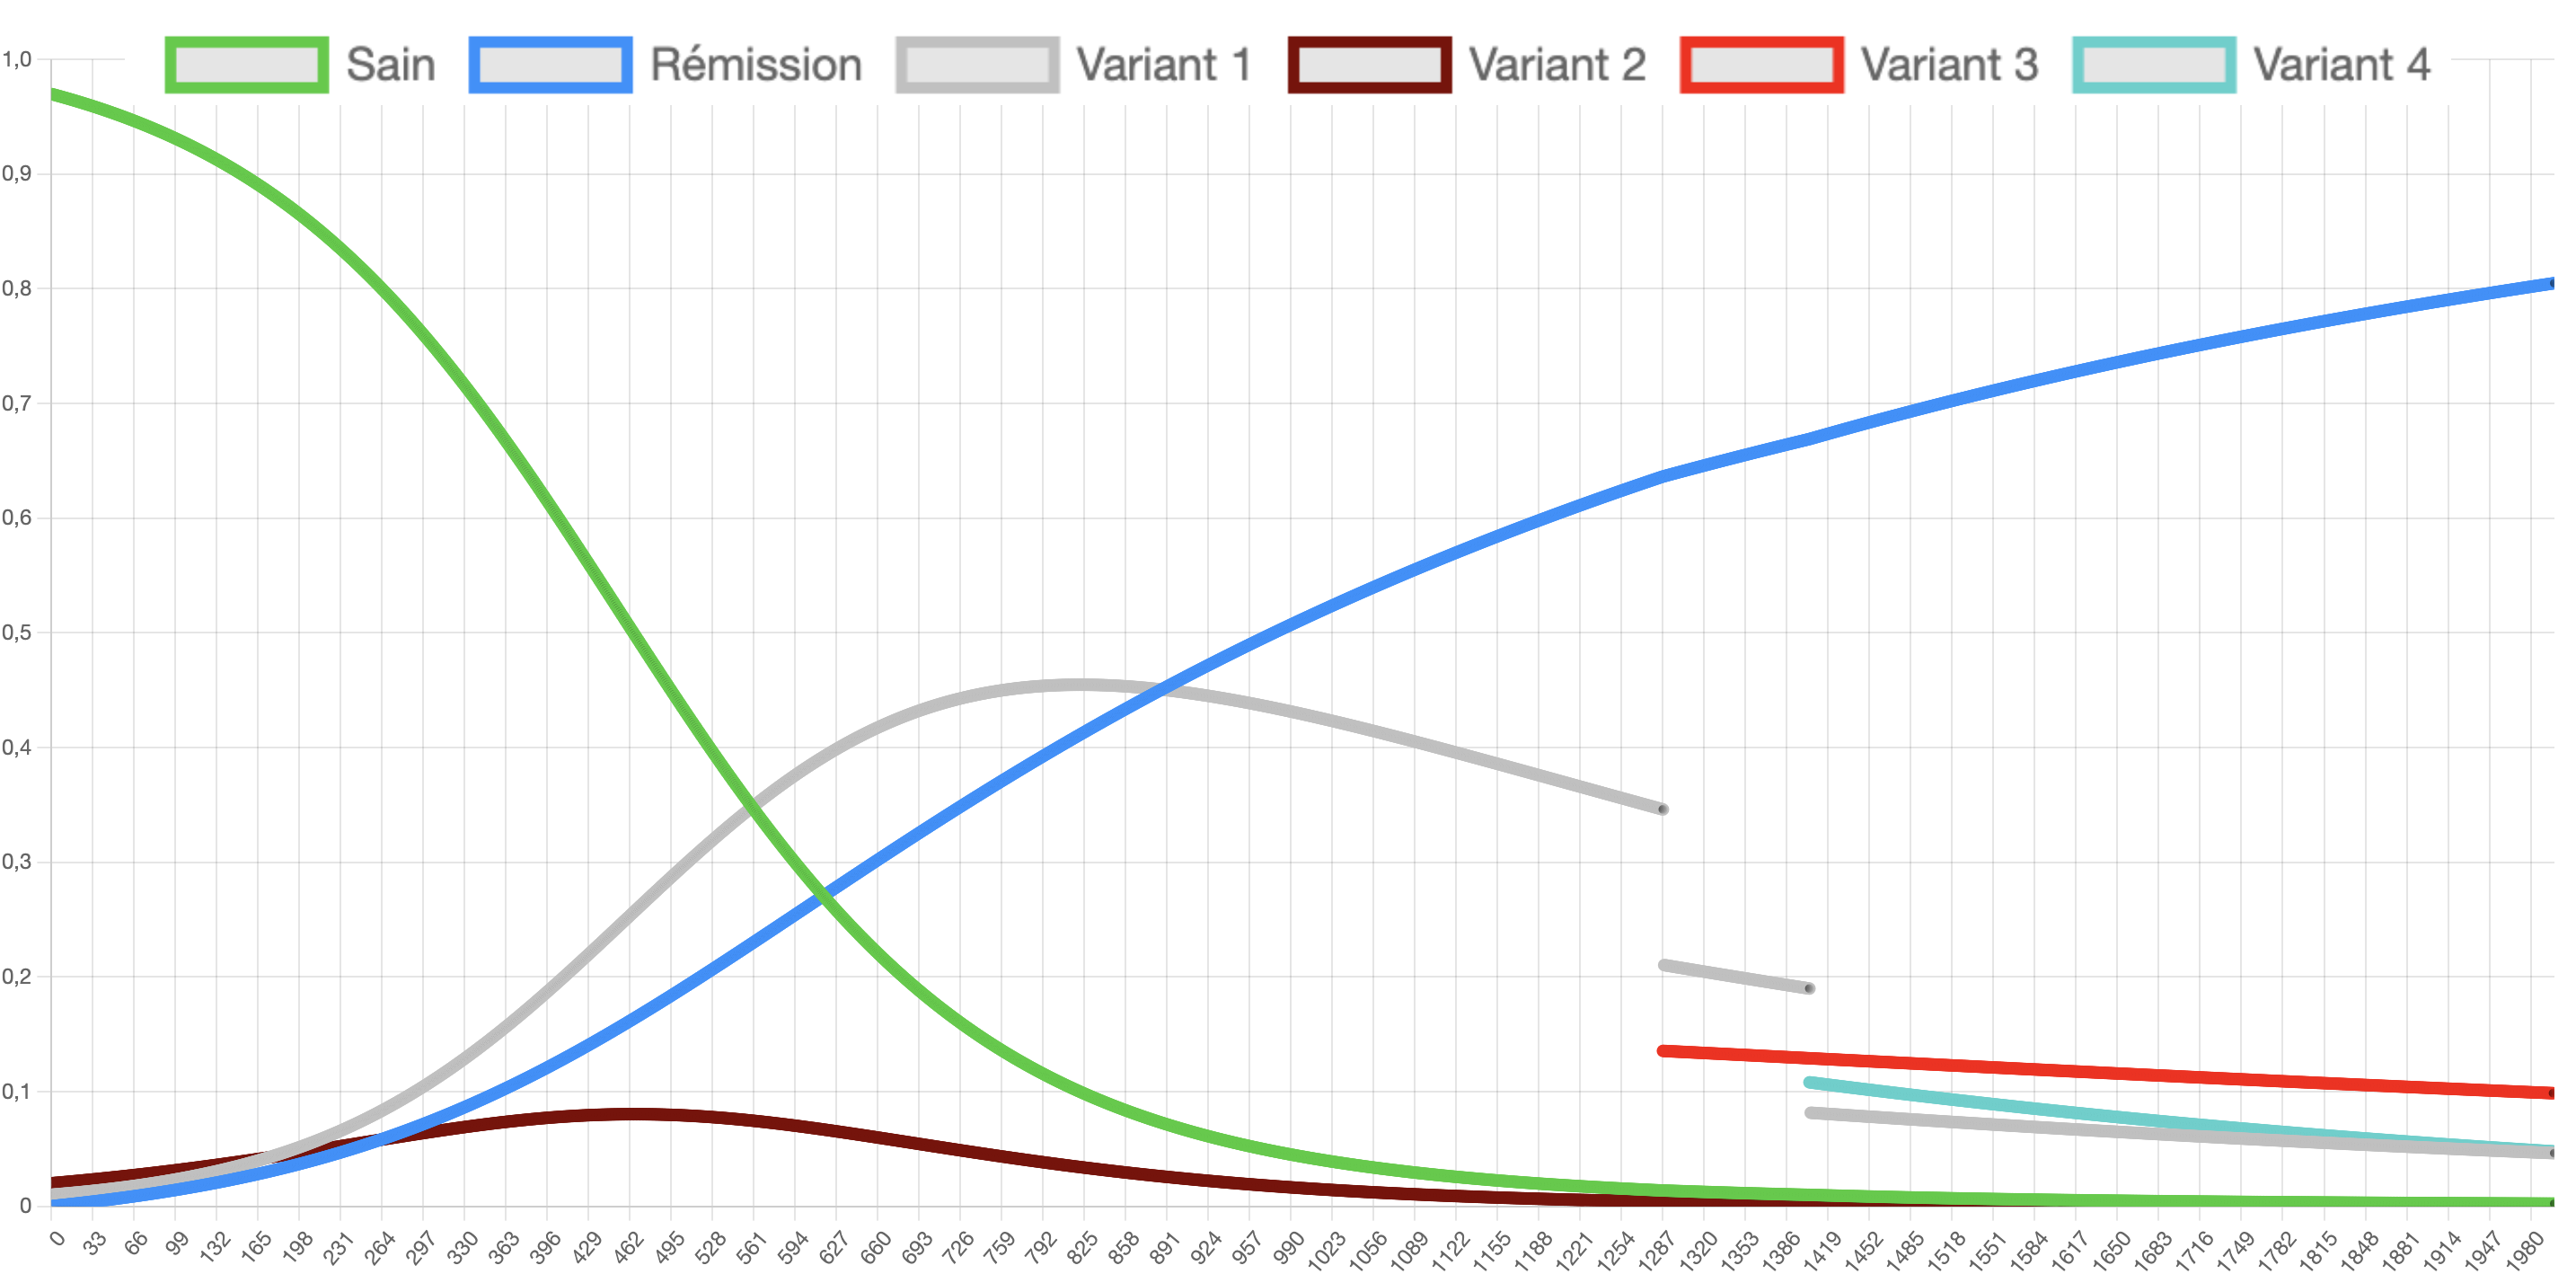
\includegraphics[width=1\linewidth]{images/Simulation2.png}
  \caption{Mutabilité du virus plus faible}
  \label{fig:sub1}
\end{subfigure}%
\begin{subfigure}{.5\textwidth}
  \centering
  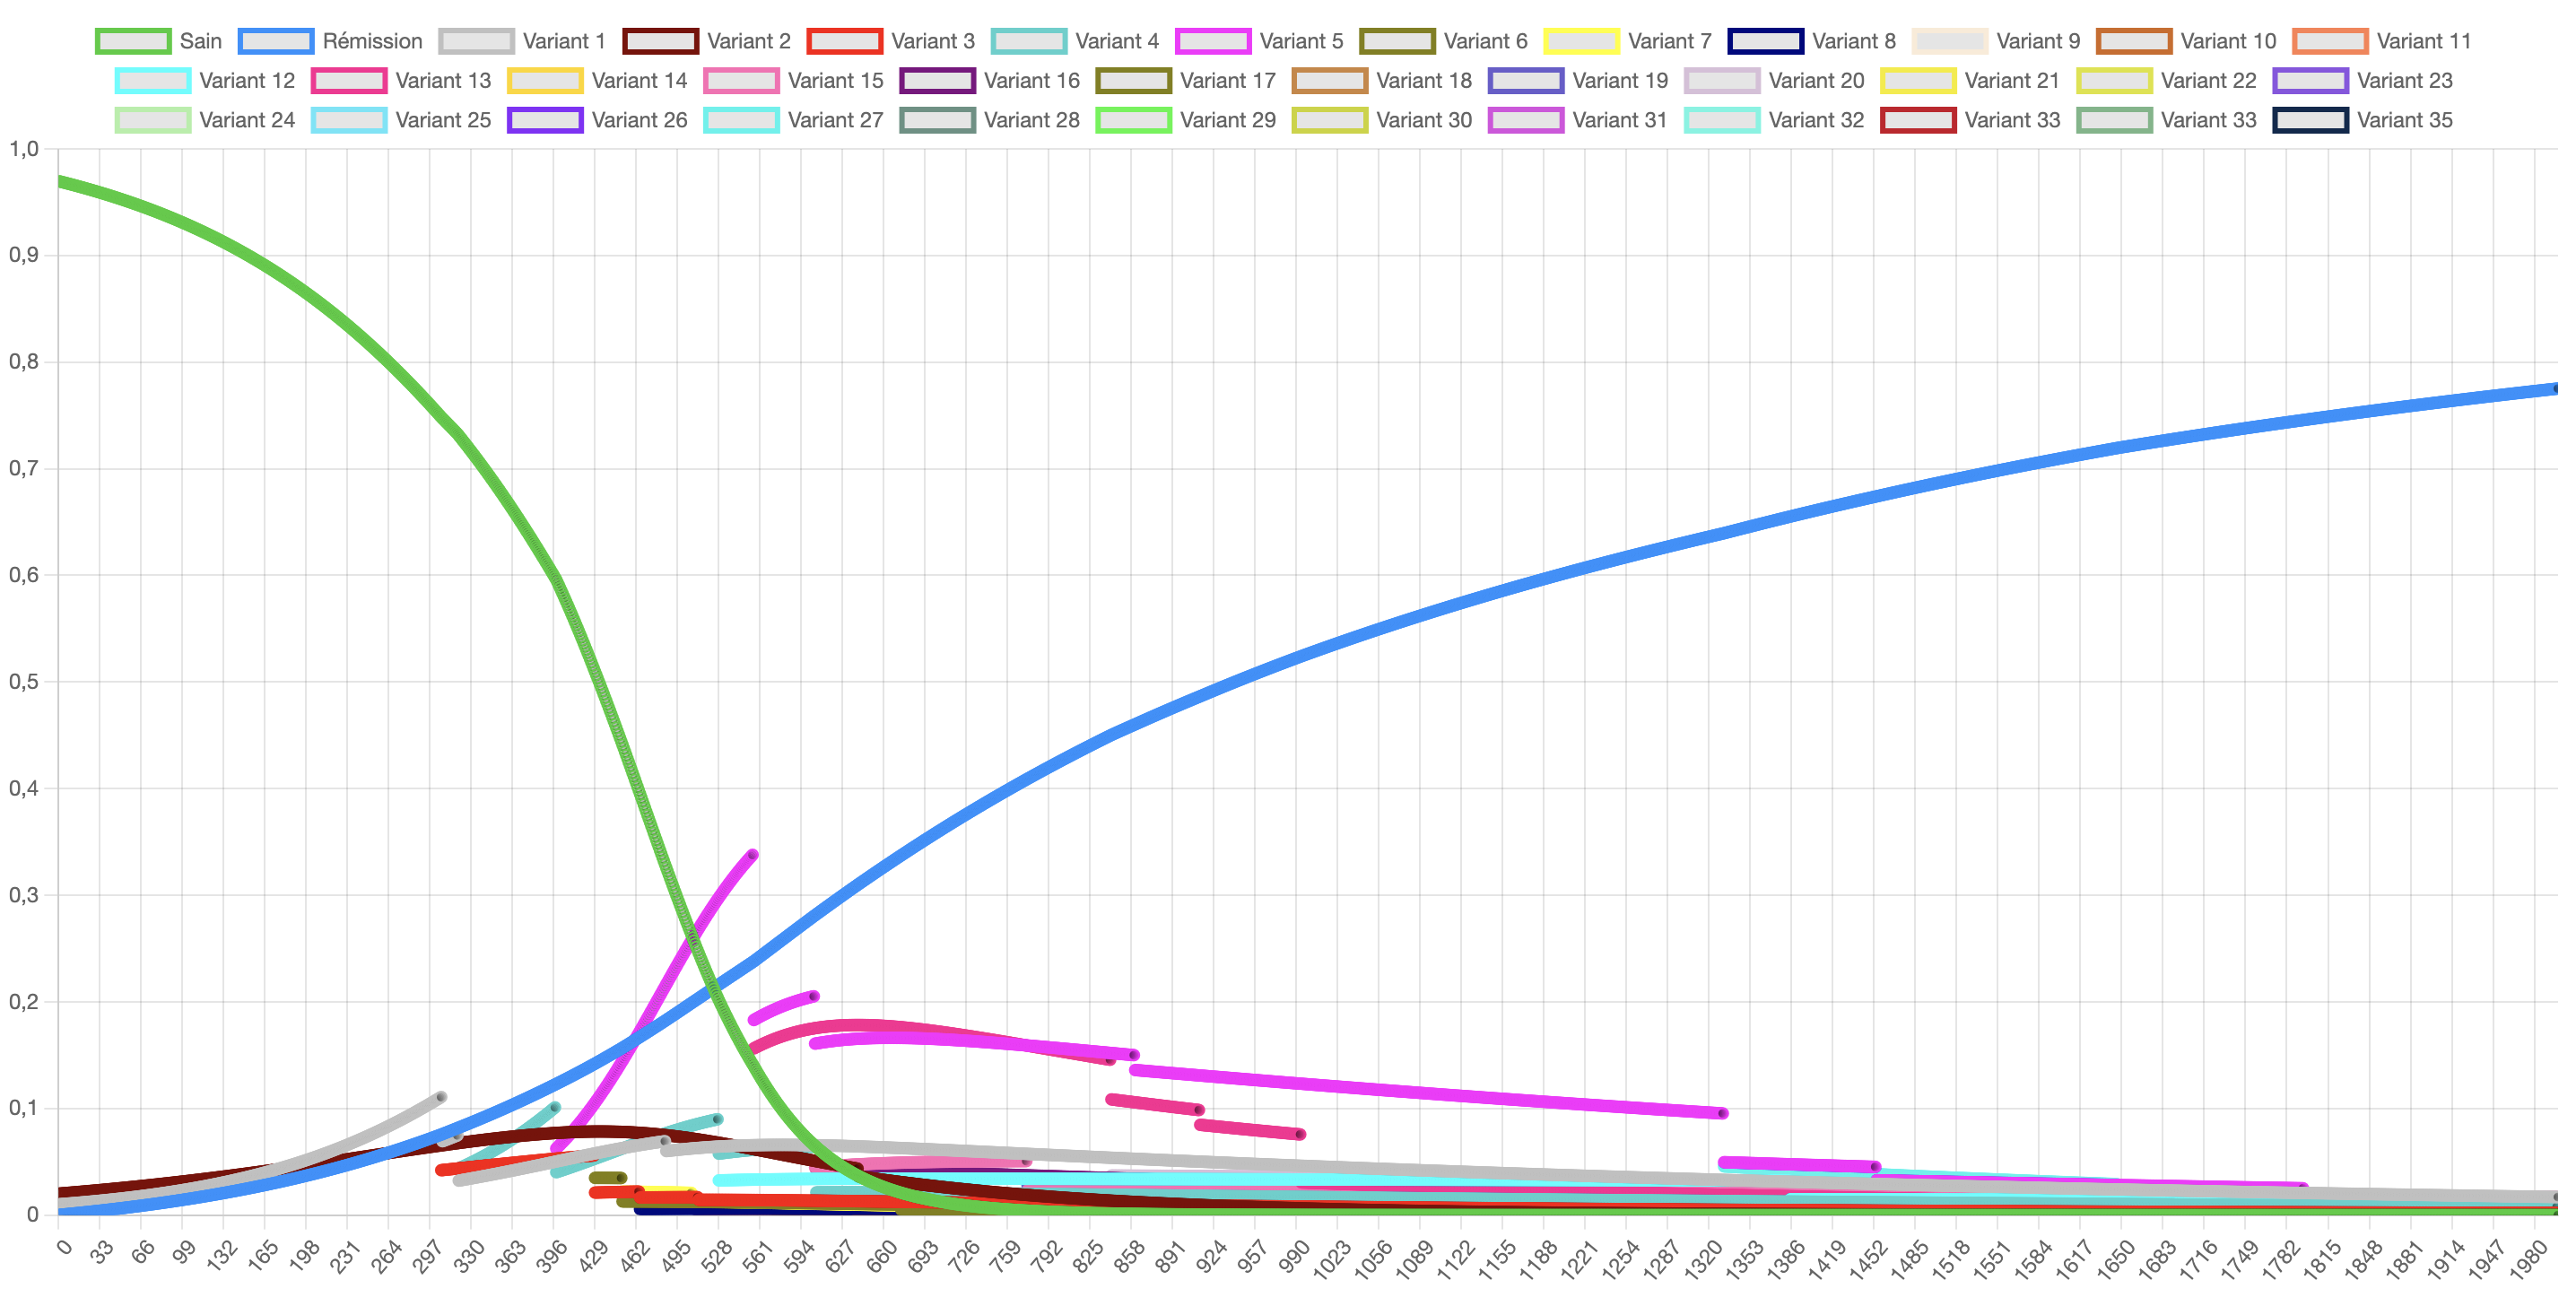
\includegraphics[width=1\linewidth]{images/Simulation2_2.png}
  \caption{Mutabilité du virus plus haute}
  \label{fig:sub2}
\end{subfigure}
\end{figure}

Pour cette simulation, on a décidé de modifier le paramètre suivant :
\begin{enumerate}
    \item Mutabilité du virus = 0,005 pour la figure (a)
    \item Mutabilité du virus = 0,05 pour la figure (b) \\
\end{enumerate}
\noindent
On remarque la création de 2 nouveaux variants. \\

Très forte domination du variant 1 sur le variant 2 bien que le taux d'infecté soit > pour le variant 2 au début de la simulation. Les taux de contagions sont les mêmes mais il y a une différence dans les taux de virulence. \\
Forte différence entre le variant 3 et le variant 4. \\ Le variant 3 est issu du variant 1, avec des critères similaires car il reste fort. \\ Le variant 4 semble avoir des caractéristiques très différentes de son parent. \\

\subsection{Influence de la force de contagion du premier variant}

\begin{figure}[h]
    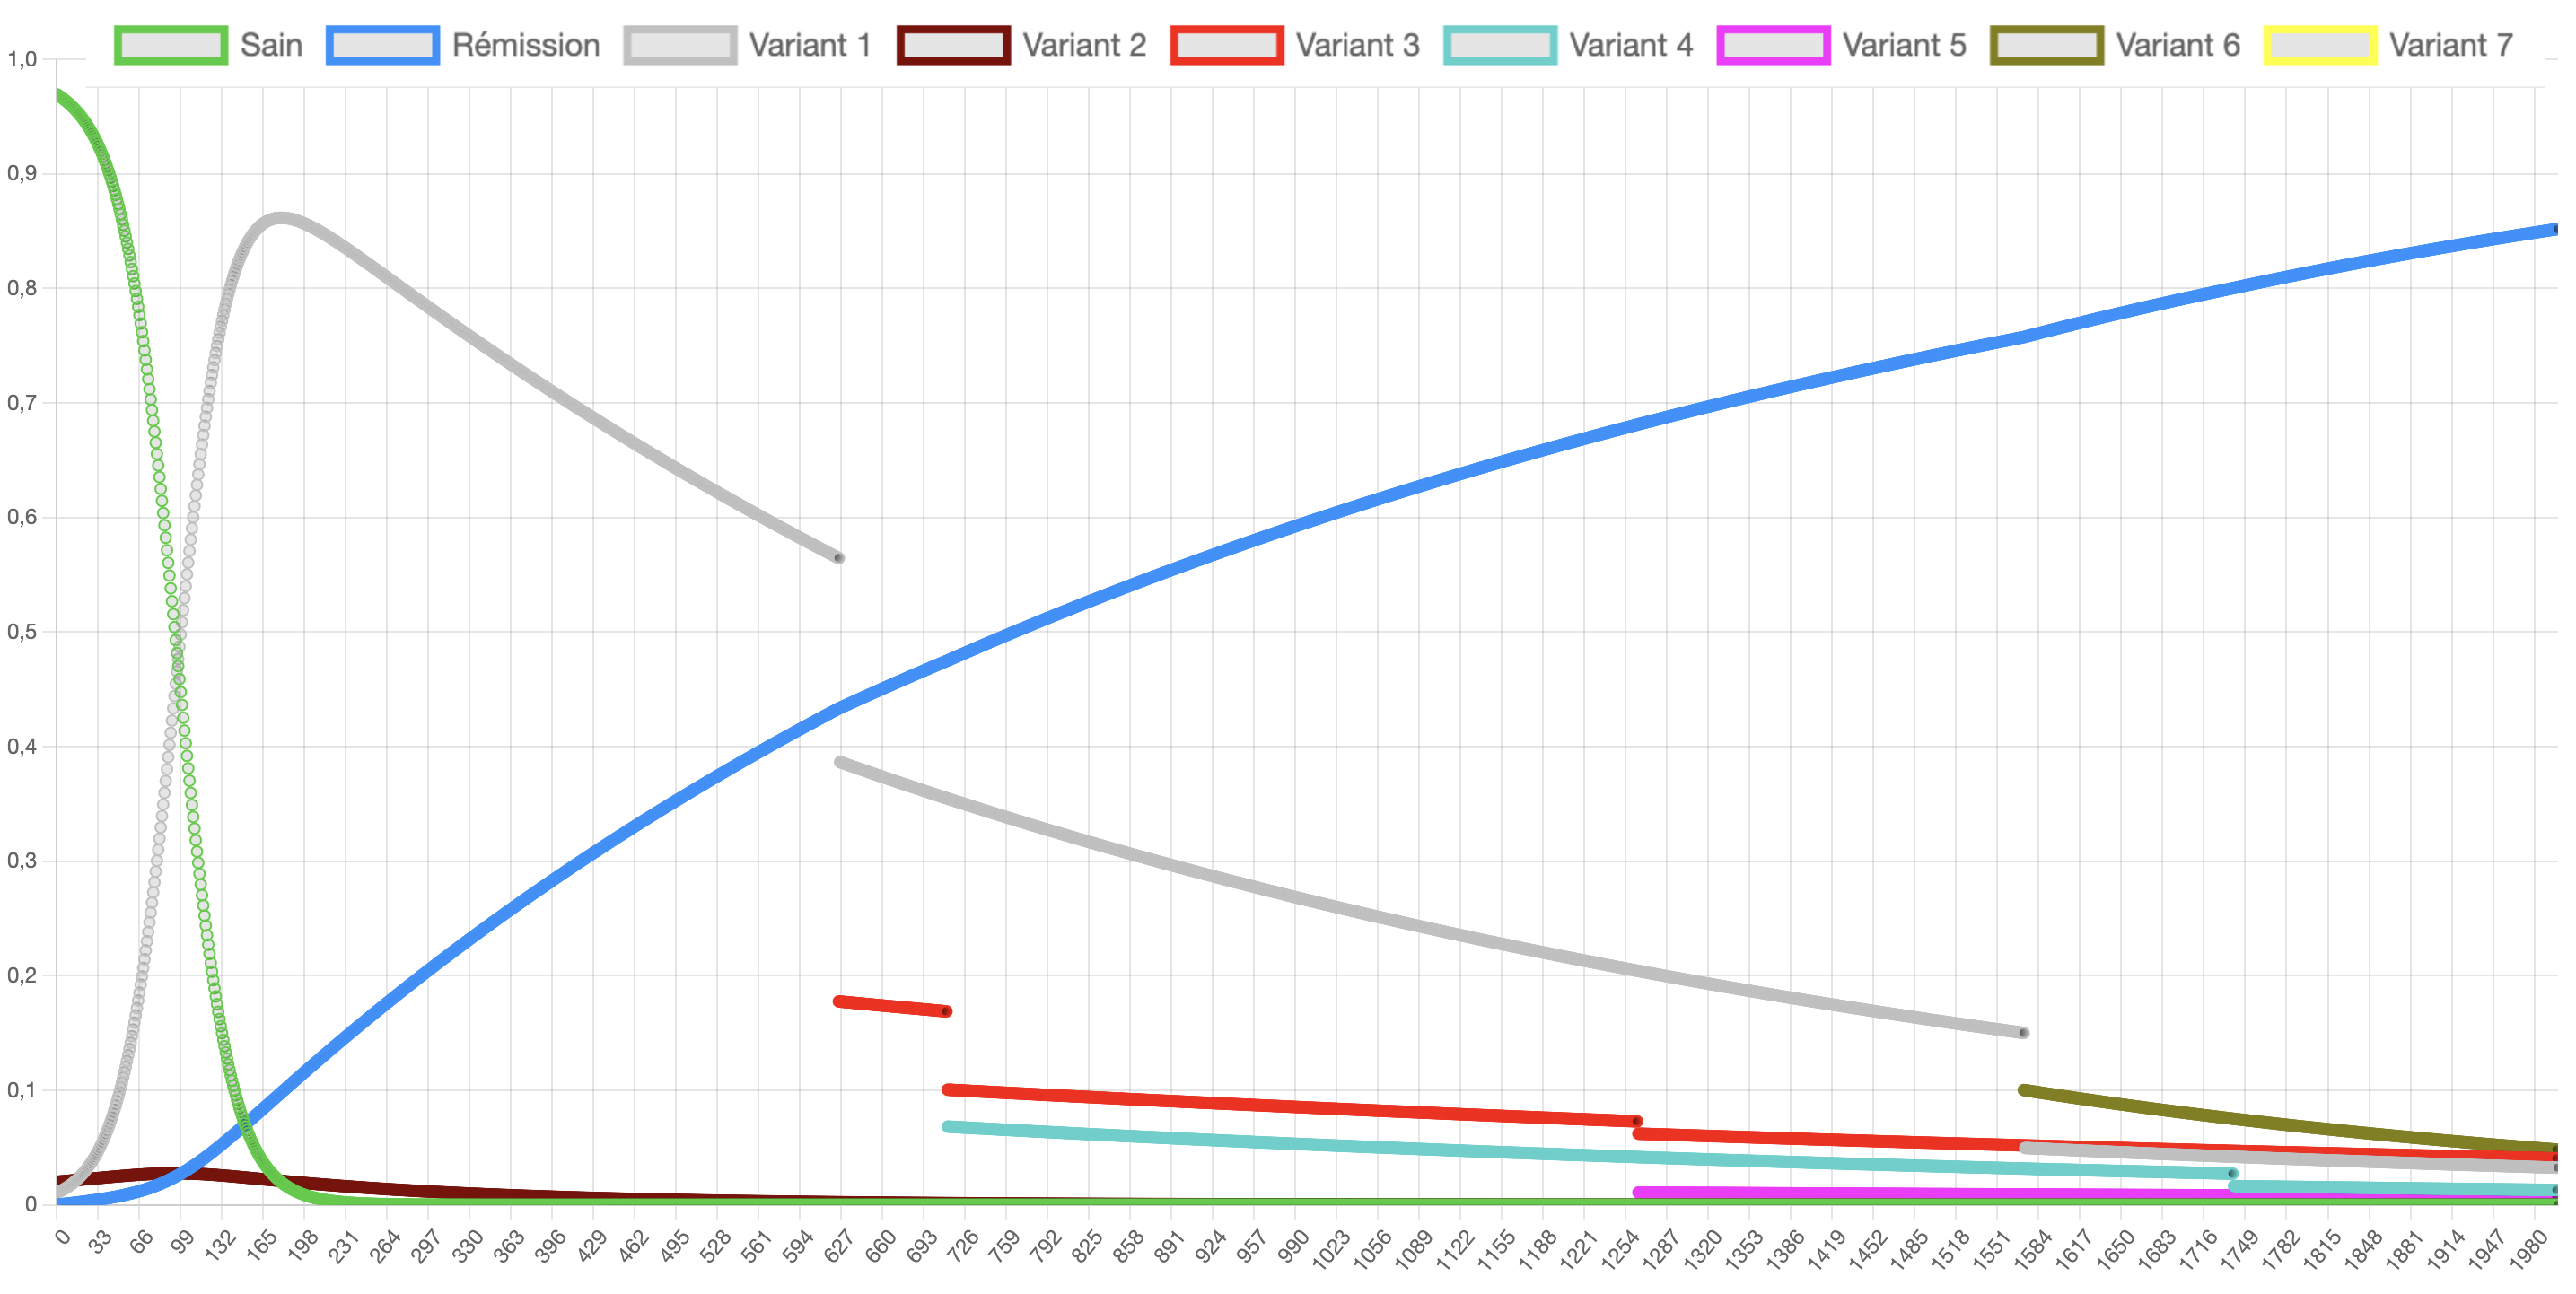
\includegraphics[width=\linewidth]{images/Simulation3.png}
    \caption{Influence de la force de contagion}
    \label{fig:simulation3}
\end{figure}

Pour cette simulation, on a décidé de modifier le paramètre suivant :
\begin{enumerate}
    \item Force de contagion du variant 1 = 0,05 \\
\end{enumerate}
\noindent
On remarque la création de 4 nouveaux variants. \\

On remarque qu'avec un taux de contagion plus élevé, le variant 1 infecte quasiment toute la population... \\

\subsection{Influence de la virulence du premier variant}


\begin{figure}[h]
    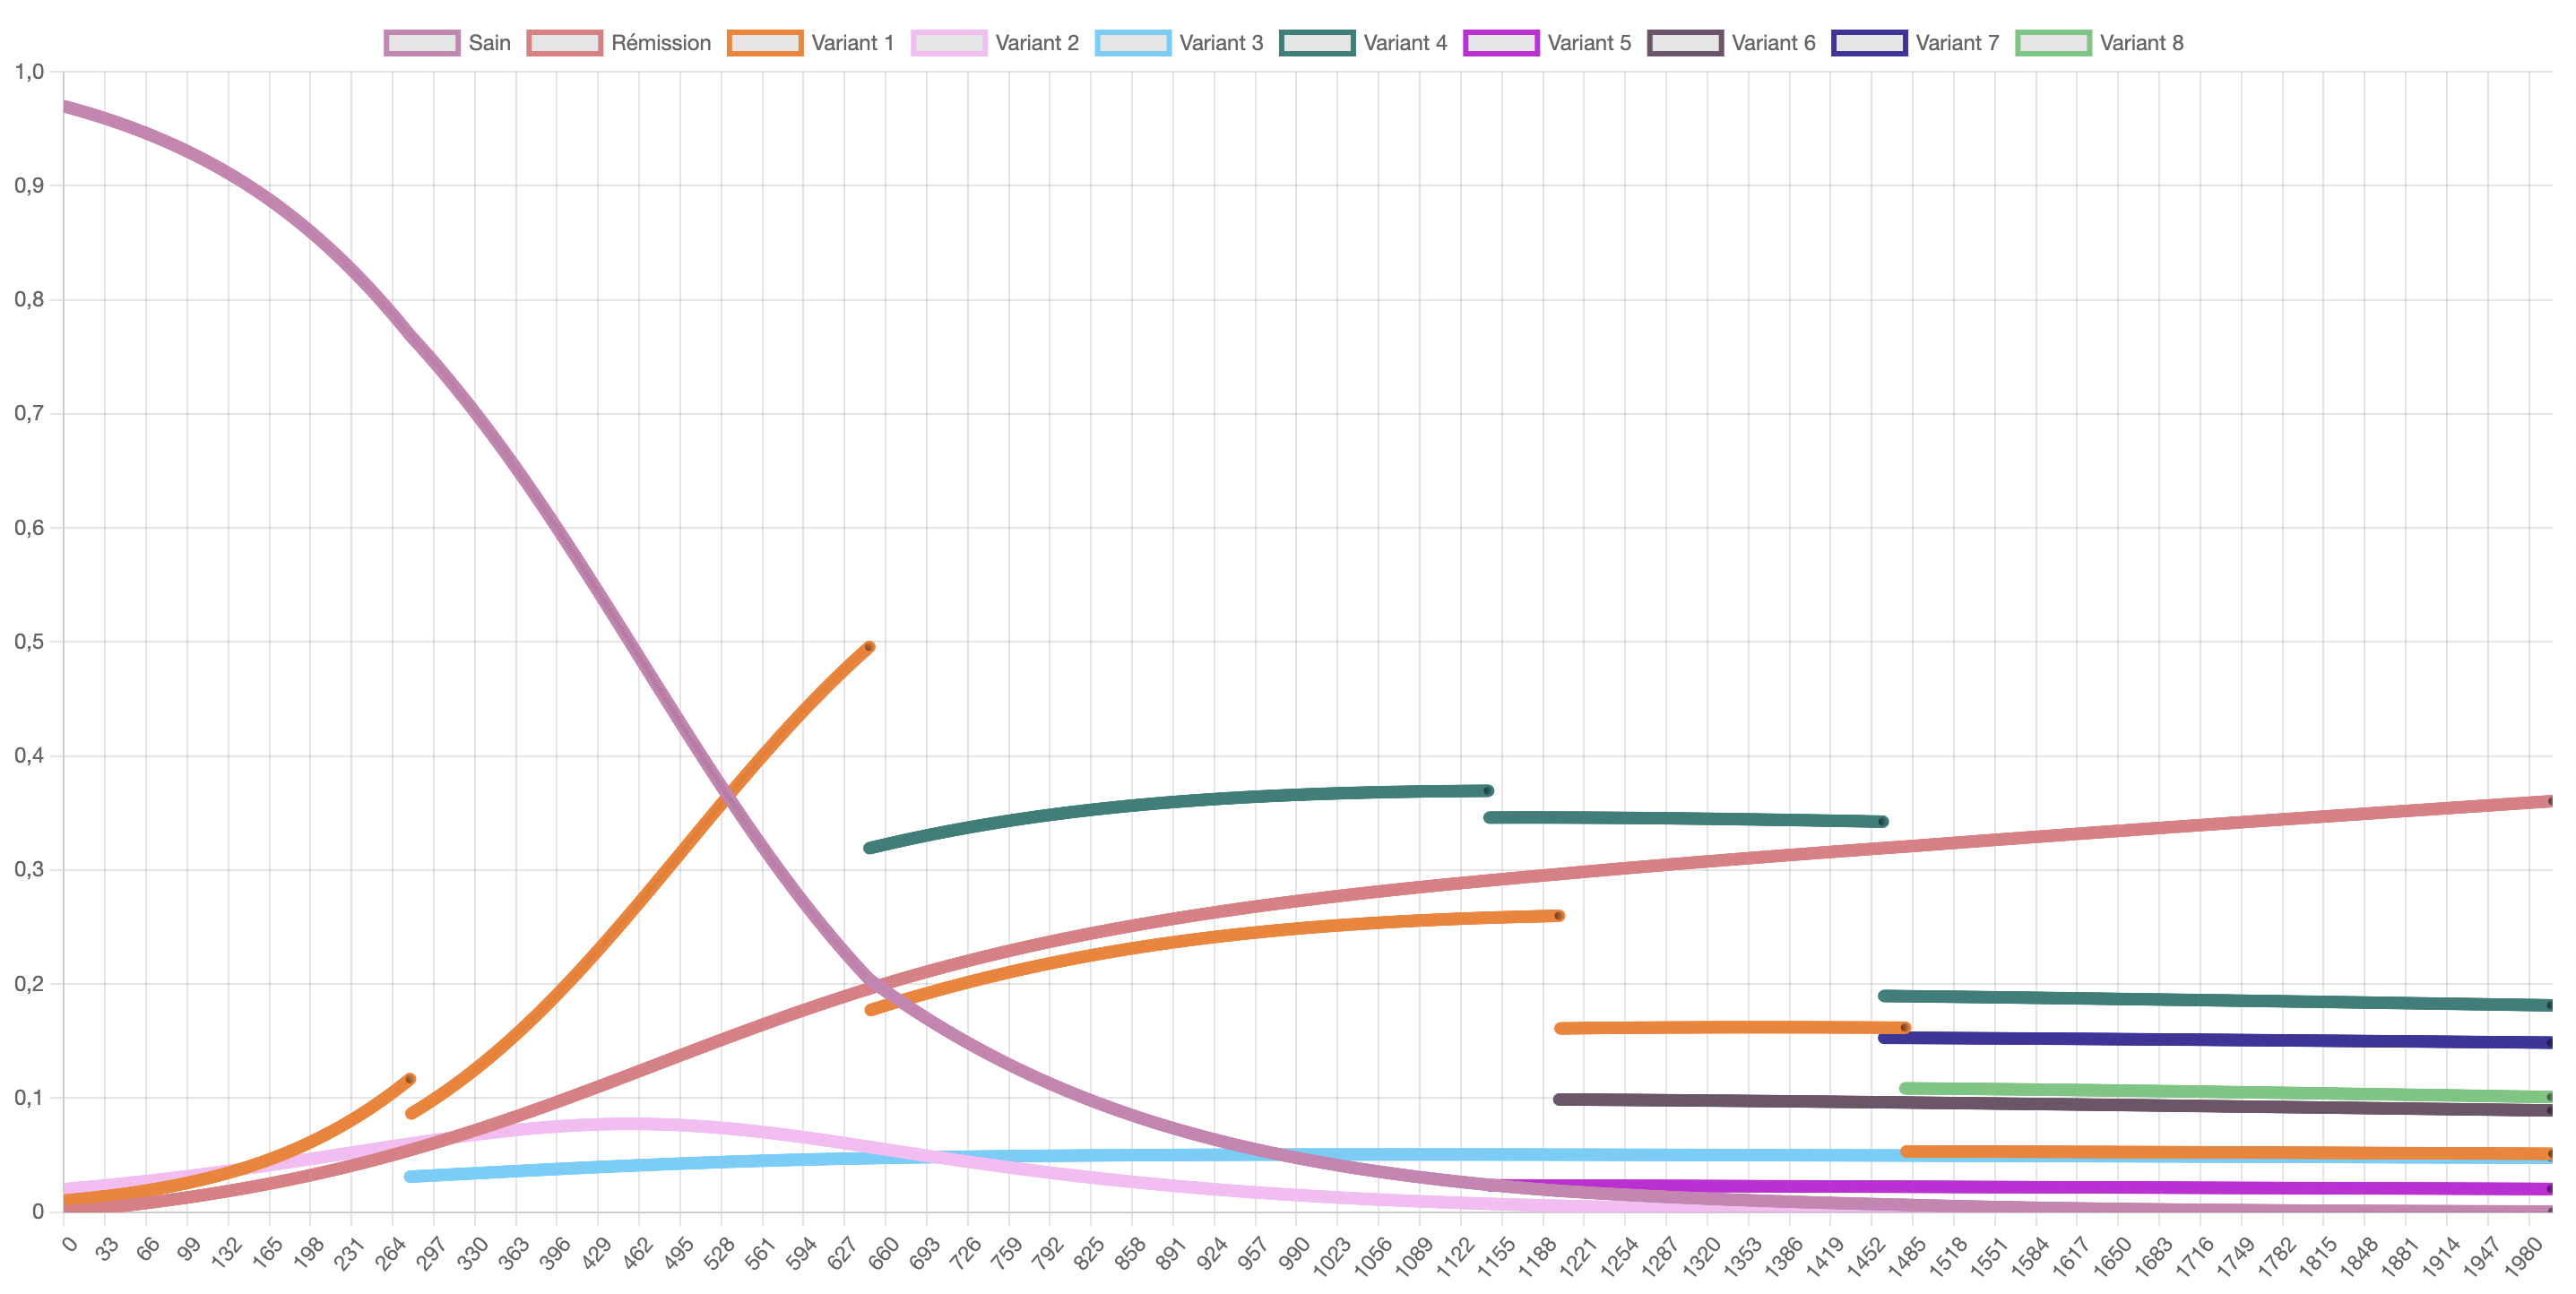
\includegraphics[width=\linewidth]{images/Simulation4.png}
    \caption{Influence de la virulence du premier variant}
    \label{fig:simulation4}
\end{figure}

Pour cette simulation, on a décidé de modifier le paramètre suivant :
\begin{enumerate}
    \item Virulence du variant = 0,0001 \\
\end{enumerate}
\noindent
On remarque la création de 6 nouveaux variants. \\

On remarque qu'avec un taux de virulence plus faible, le variant 1 infecte une bonne partie de la population et le taux de rémission reste faible après 2000j. \\
De plus le viriant 4, issu du variant 1, est plus fort que son parent à la fin de la simulation. \\
Inexistance du variant 2.


\subsection{Simulation pour avoir un variant gagnant sur le taux de rémission}

\begin{figure}[h]
    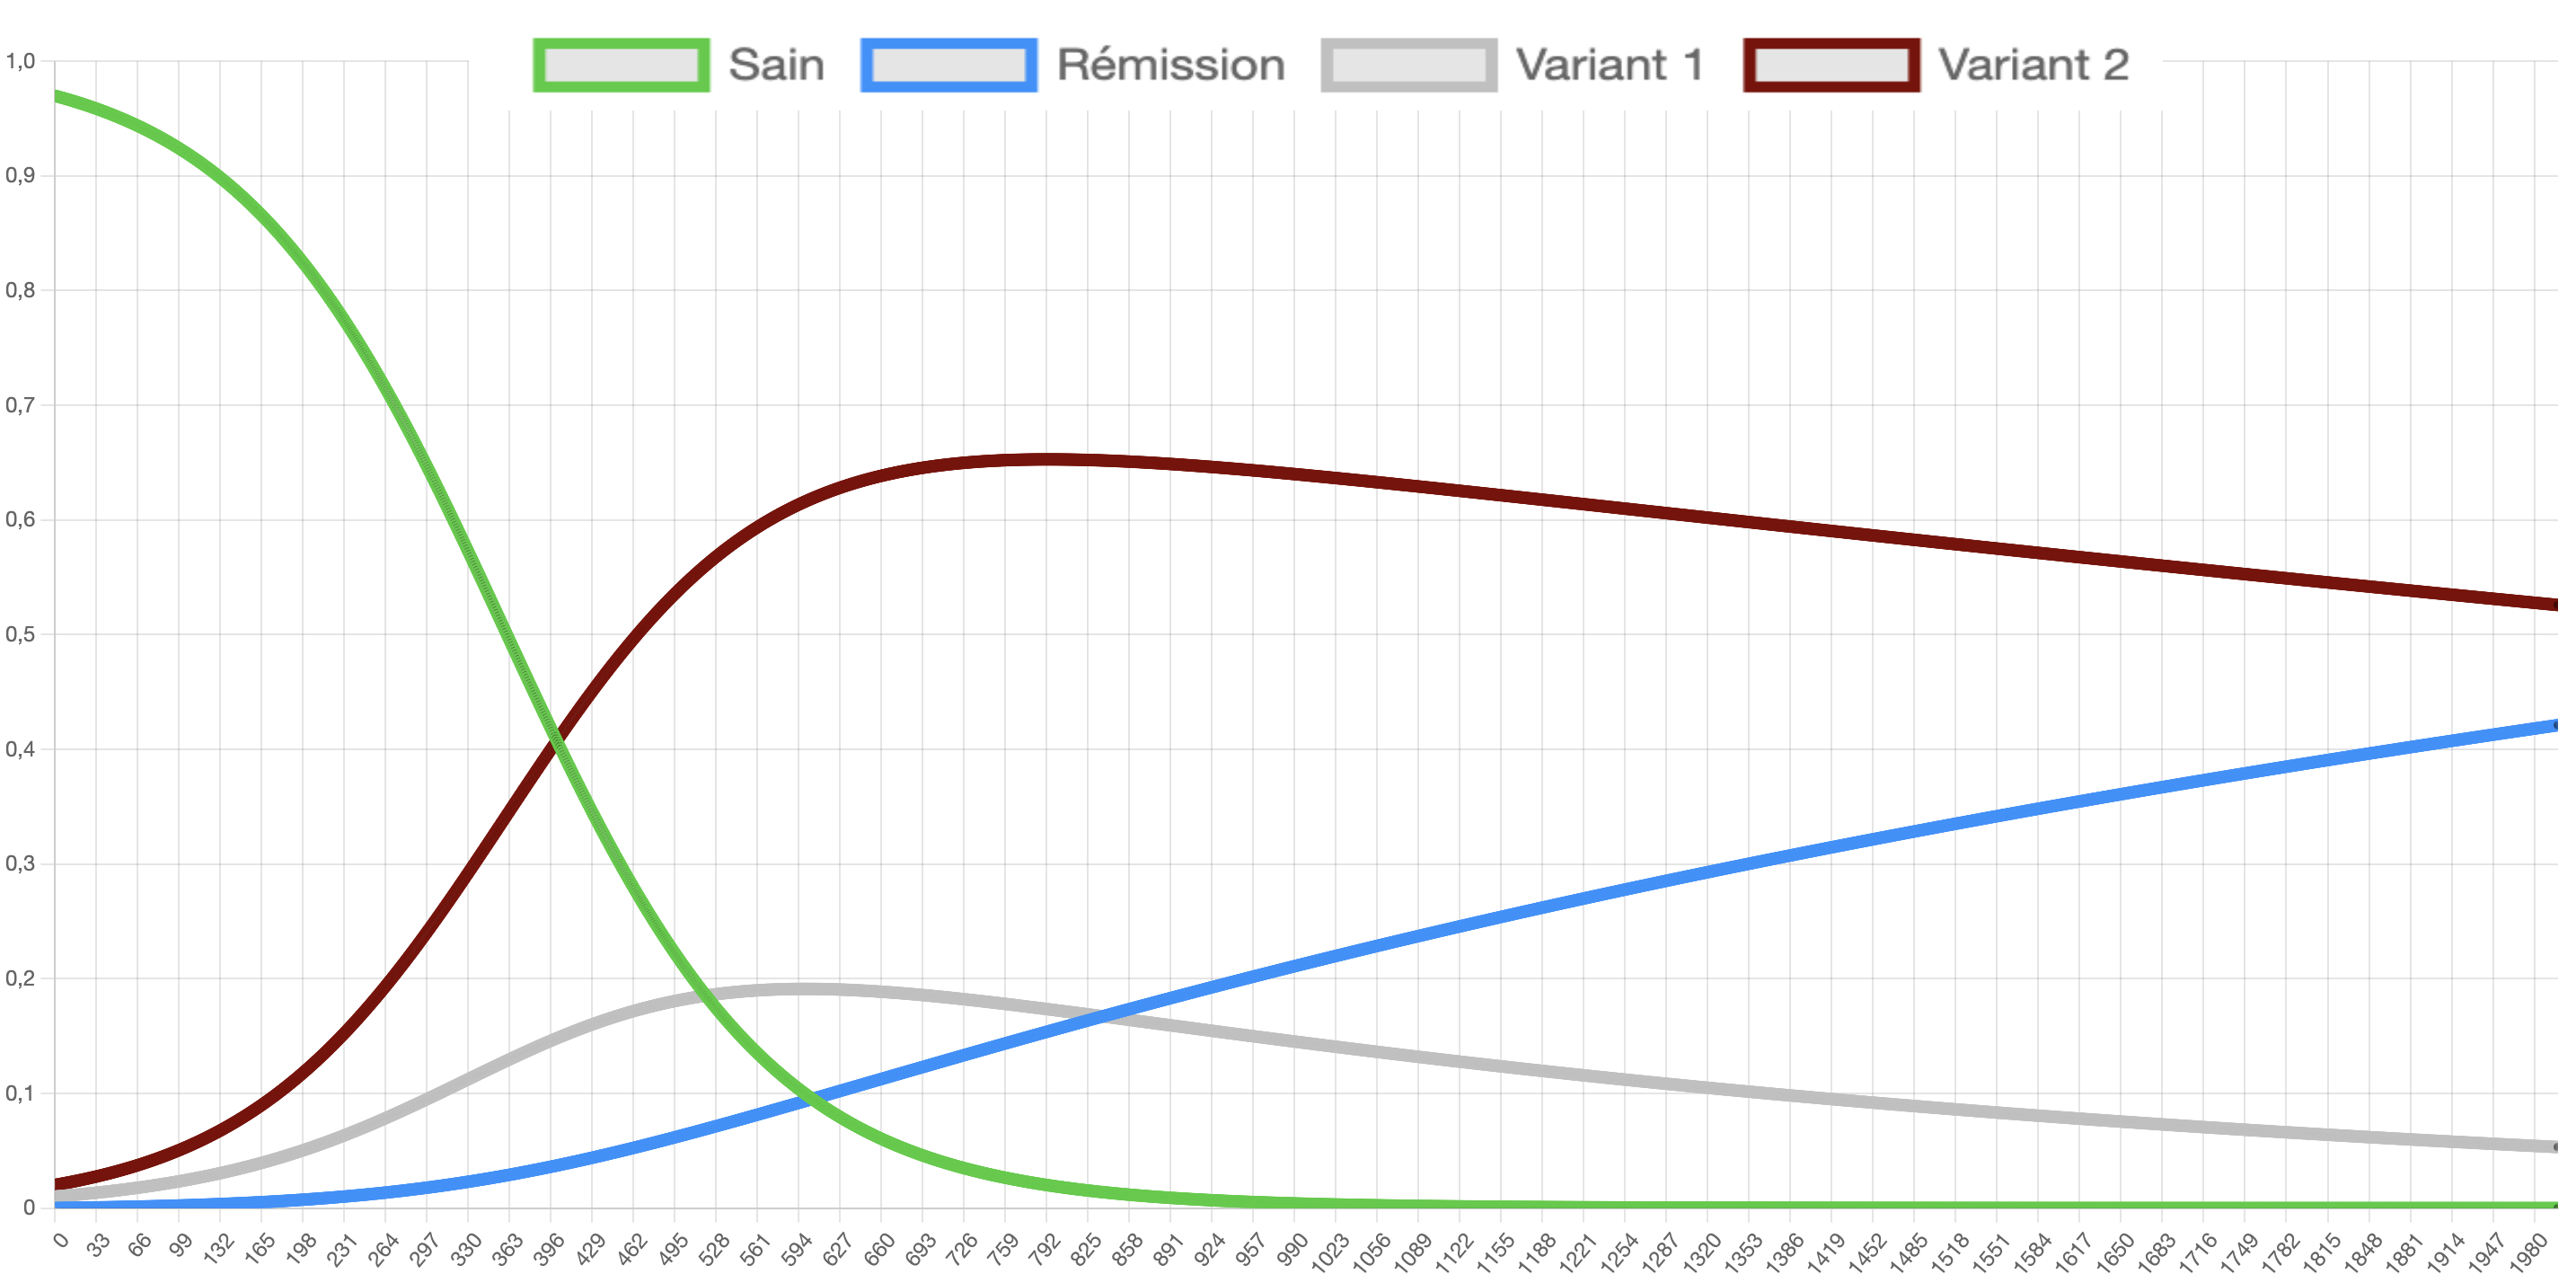
\includegraphics[width=\linewidth]{images/Simulation5.png}
    \caption{Simulation pour avoir un variant gagnant sur le taux de rémission}
    \label{fig:simulation5}
\end{figure}

Pour cette simulation, on a décidé de modifier les paramètres suivants :
\begin{enumerate}
    \item Mutabilité du virus = 0,0001
    \item Virulence du variant 2 = 0,0002
\end{enumerate}


\section{Discussion des résultats}

Dans cette partie, on s'intéressera à l'interprétation des résultats de chaque simulation afin d'en déduire les paramètres les plus intéressants pour le dévéloppement de nos variants.



On remarque que les nouveaux variants entrainent une coupure dans les courbes des variants dont ils sont issus. \\
En effet, le taux de personnes infecté par un variant est issu du taux de personne infecté par le variant parent. \\
Nous avons décidé de faire en sorte que la création d'un variant affecte un grand nombre de la population du variant parent afin d'avoir des résultats intéressant directement. Si nous avions décidé de faire muter qu'une petite partie de notre population, nous aurions eu des difficultés à étudier le développement des variants. En effet, dans la réalité, il y a des millions de variants qui naissent chaque jour mais seulement un faible nombre survit. Pour des raisons de performances, nous ne pouvons pas modéliser des millions de variants.

L'effet de la durée de la simulation sur les variants (à la fin, est-ce qu'un variant domine ou alors est-ce que tout le monde est remis ?) \\

Si pas de simulation faisant varier la virulence du variant -> parce que l'on ne peut pas tuer les gens. Donc la virulence n'est finalement pas super intéressante ?

Sur un temps T défini, résultats :\\
- apparition de nouveaux variants par mutations, nombre final de variants\\
- impact sur les personnes saines, en rémission\\
- mutation qui prend le dessus sur son variant père (extraire caractéristiques)\\

\section{Conclusion}

Le comportement de l'épidemie de la COVID-19 est-il influencé par la circulation, la mutation et l'interaction des variants ?
A partir de nos simulations, on a conclu que la circulation et la mutation des variants permet a un virus d'infecter la quasi-totalité de la population très rapidement. L'interaction entre les variants permet de conclure que si le taux de virulence est faible, un variant enfant peut contaminer plus de monde q'un variant parent. \\

Concernant les perspectives d'améliorations, nous pouvons envisager :
\begin{enumerate}
    \item La gestion du nombre de variants de départ. Cela permettrait d'approfondir encore plus les possibilité de simulation.
    \item L'ajout d'une notion de graine lié au randomisateur. Avec cela, on peut s'assurer que les résultats obtenus sont toujours identiques pour les mêmes paramètres bien que l'on utilise un système se basant sur une forme d'aléatoire.
    \item La possibilité de se faire infecter par plusieurs variants en même temps.
    \item La possibilité de se faire infecter une nouvelle fois après guérison d'un autre variant.
    \item L'ajout d'une notion de vaccination, les personnes saines pourraient être vaccinées ou non ainsi que les personnes remises.
    \item Ajouter des détails au moment de la création d'un variant (notamment sur le fait de savoir s'il est né avec des paramètres très différents de son parent.).
    \item Enfin, il manque une notion principale, le fait de pouvoir décéder du variant. Dans nos simulations, la population est soit saine, soit en rémission soit infecté mais elle ne peut pas être infecté puis décédée.
\end{enumerate}

\section{Référence}

Marquioni, V., & de Aguiar, M. (2021). Modeling neutral viral mutations in the spread of SARS-CoV-2 epidemics. PLOS ONE, 16(7), e0255438. doi: 10.1371/journal.pone.0255438


\end{document}
